\subsubsection{Toy Example}
\noindent
Say we wish to maximize $f(x,y) = x+y$ subject to the constraint $g(x,y) = x^2 + y^2 = 1$.
We can do this y finding the C-level curve that is tangent to our constraint, as this curve will have the extrema.\\
At this point, $\nabla f$ will be in the same direction as $\nabla g$.
That is,
\begin{equation*}
	\begin{cases} 
		f_x = \lambda g_x \\ 
		f_y = \lambda g_y
	\end{cases}.
\end{equation*}
We also add the constraint itself, $g(x,y)$ equals some constant $k$, giving us a system of equations
\begin{equation*}
	\begin{cases}
		f_x = \lambda g_x \\ 
		f_y = \lambda g_y \\ 
		g(x,y)=k 
	\end{cases}.
\end{equation*}

\begin{figure}[H]
	\centering
	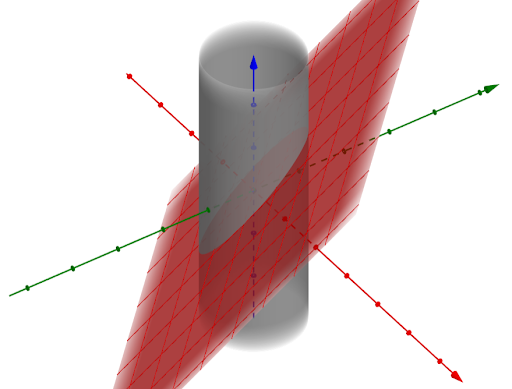
\includegraphics[width=0.33\textwidth]{./differentialMultivariableCalculus/lagrange_slice.png}
	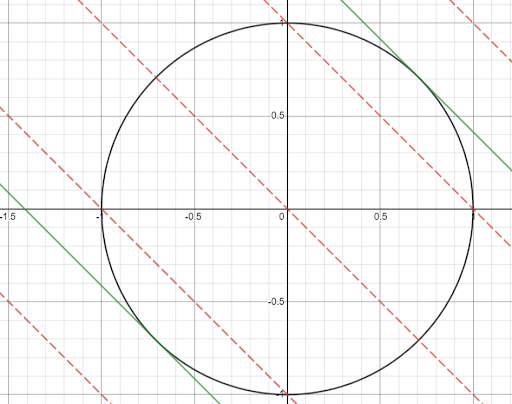
\includegraphics[width=0.33\textwidth]{./differentialMultivariableCalculus/lagrange_curves.png}
	\caption{Extremas when the constraints (black) are tangent to the level curves.}
\end{figure}